\documentclass[tikz,border=3mm,multi=tikzpicture]{standalone}
\usepackage[utf8]{inputenc}
\usepackage[T1]{fontenc}
\usepackage{helvet}
\renewcommand{\familydefault}{\sfdefault}
\usepackage{tikz}
\usetikzlibrary{arrows.meta,positioning,calc}
\begin{document}

\tikzset{every node/.append style={font=\sffamily\small}}

% TikZ 1
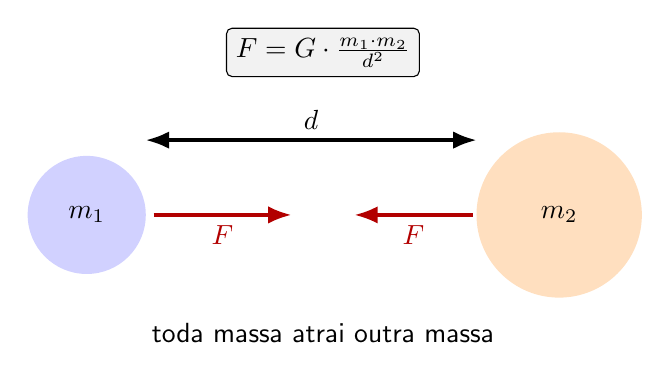
\begin{tikzpicture}[>=Latex]
  \fill[blue!18] (-3,0) circle (0.75);
  \fill[orange!25] (3,0) circle (1.05);
  \node at (-3,0) {$m_1$};
  \node at (3,0) {$m_2$};
  \draw[very thick,<->] (-2.25,0.95) -- (1.95,0.95) node[midway,above] {$d$};
  \draw[very thick,->,red!70!black] (-2.15,0) -- (-0.4,0) node[midway,below] {$F$};
  \draw[very thick,->,red!70!black] (1.9,0) -- (0.4,0) node[midway,below] {$F$};
  \node[align=center,below] at (0,-1.25) {toda massa atrai outra massa};
  \node[draw,rounded corners=2pt,fill=gray!10,align=center,above] at (0,1.75)
    {$F = G \cdot \frac{m_1 \cdot m_2}{d^2}$};
\end{tikzpicture}

% TikZ 2
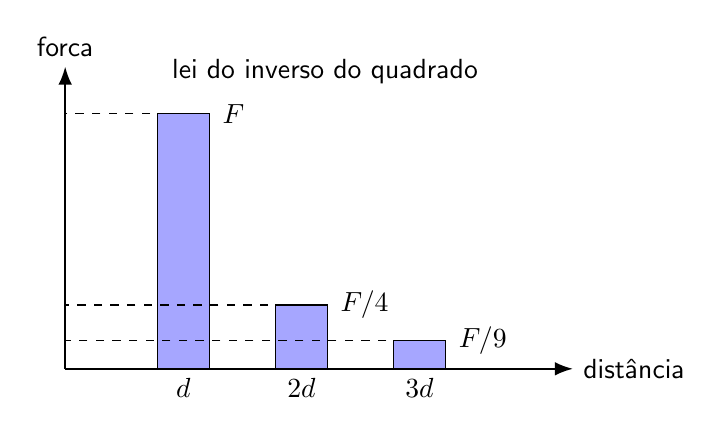
\begin{tikzpicture}[x=1.5cm,y=1.2cm,>=Latex]
  \draw[->,thick] (0,0) -- (4.3,0) node[right] {distância};
  \draw[->,thick] (0,0) -- (0,3.2) node[above] {forca};
  \foreach \x/\lab in {1/$d$,2/$2d$,3/$3d$}{
    \draw[fill=blue!35] (\x-0.22,0) rectangle (\x+0.22,{2.7/(\x*\x)});
    \node[below] at (\x,0) {\lab};
  }
  \node[right] at (1.25,2.7) {$F$};
  \node[right] at (2.25,0.675) {$F/4$};
  \node[right] at (3.25,0.3) {$F/9$};
  \draw[dashed] (1,2.7) -- (0,2.7);
  \draw[dashed] (2,0.675) -- (0,0.675);
  \draw[dashed] (3,0.3) -- (0,0.3);
  \node[align=center] at (2.2,3.15) {lei do inverso do quadrado};
\end{tikzpicture}

\end{document}
